\subsubsection{BER bounds on UEP fountain codes}
Another interesting point of view is the one given in \cite{Yue2014}, where the main aim is not optimizing the general success probability, but instead defining an upper and lower \gls{ber} bound in the case of \gls{uep} for \gls{dnc} schemes over Rayleigh fading channels.

Distributed coding is an efficient channel coding strategy that improves the transmission reliability of cooperative communication networks. In many real-life applications, however, source nodes require a form of unequal protection from errors, instead of the Equal counterpart extensively addressed in \cite{Pang2012}, and this is at the origin of the design of a form of fountain codes called \gls{uep} fountain codes. In \cite{Yue2014}, the authors adopt the wieghted method to realize such codes, which consists in dividing the transmission data into several protection groups according to their protection requirements and assigning corresponding protection weights.

\paragraph{The system model} \label{sec:relayBER}
The system model in the paper is the following: consider a \gls{wsn} where a single destination node (the sink) communicates with $K$ source nodes through a common relay network with $N$ relay nodes. The authors also add the assumption that the $K$ source nodes belongs to $T$ source groups with different error protection requirements. The data delivery from the source node to the sink is then carried out in three phases:
\begin{itemize}
  \item \textit{The broadcast phase} - In which the information sequence of each source node is appended with a header, containing the protection weight $\omega_\tau$, and a \gls{crc} code, to form a data packet;
  \item \textit{The Relay phase} - in which each relay node decodes the received data packets and selects uniformly at random a fixed number $d$ of them. Among the selected data, $d^\tau$ of them are from the source node in the protection group $\tau$ and the degree distribution $\mu^\tau(x)$ is generated by applying the \gls{uep} \gls{dnc} guidelines to the degree distribution $\mu(x)$;
  \item \textit{The data recovery phase}
\end{itemize}
Moreover, the benefits of a relay-type network structure for a \gls{wsn} is largely investigated in the work of Comaniciu \textit{et al.}, where several relay solutions are analised and compared in the specific combination of LT codes instead of \gls{rl} ones \cite{Comaniciu2011}.\\
Finally, in the model there hase been defined two main protection level groups (for sake of simplicity), a \gls{hep} and a \gls{lep} group.

\paragraph{The \gls{ber} bounds}
With these premises we can present here the \gls{ber} bounds on the bit error probability for the \gls{hep} group, while the bounds for the \gls{lep} group can be easily obtained by simple switch of the terms $K_H$ and $K_L$ and substitution of the other parameters of the protection group. Considering a \gls{uep} \gls{dnc} based on fountain codes with degree distribution on \gls{hep} $\mu_{w(ch)^H}$, $K_H$, $K_L$, number of data packets collected $Q$, the error sequence $\mathbf{e}$, the $K\times Q$ matrix $\mathbf{G}$ and Hamming weight $w(\cdot)$, then the \gls{ber} performance for the protection group \gls{hep} with \gls{ml} decoding over Rayleigh fading channels can be upper bounded by $\xi_U^F < min\{1,\xi_U\}$, where $\xi_U$ is given by:
\begin{align}
\centering
  \xi_U & = \sum_{k=1}^K\sum_{k_h = max\{0,k-K_L\}}^{min\{k,K_H\}}\frac{k_H}{K_H}\binom{K_H}{k_H}\binom{K_L}{k - k_H}\\
   \cdot\biggl\{\biggl[\sum_{w(\mathbf{c}_H)}\mu_{w(\mathbf{c}_H)}^H\zeta(w(\mathbf{c}_H),&w(\mathbf{e})) = k,w(\mathbf{e}_H) = k_H)\biggr]^Q+P_r(\mathbf{eG} \neq \mathbf{0},w(\mathbf{e} = k, w(e_H)) = k_H)\biggr\}
\end{align}
At the same time, the same \gls{ber} performance can be lowerbounded by $\xi_L^F > max\{0,\xi_L\}$, where $\xi_L$ is given by:
\begin{align}
\centering
  \xi_L & = \sum_{k_h = max\{0,1-K_L\}}^{min\{1,K_H\}}\frac{k_H}{K_H}\binom{K_H}{k_H}\binom{K_L}{1 - k_H}\\
   \cdot\biggl\{\biggl[\sum_{w(\mathbf{c}_H)}\mu_{w(\mathbf{c}_H)}^H\zeta(w(\mathbf{c}_H),&w(\mathbf{e})) = 1,w(\mathbf{e}_H) = k_H)\biggr]^Q+P_r(\mathbf{eG} \neq \mathbf{0},w(\mathbf{e} = 1, w(e_H)) = k_H)\biggr\}
\end{align}
The proof of the previous results can be found in \cite{Yue2014}.

\paragraph{Results}
\autoref{fig:berLT} (a) and (b) show the upper and lower \gls{ber} bounds at an average $E_s/N_0 = 0.9dB$: as it is evident, the upper and lower bounds become asymptotically tight as the expanding coefficient $\eta$ grows. Moreover, the \gls{ber} performance of the \gls{hep} group is better, compared to the Equal protection design, while the \gls{lep} group is only slightly worse.\cite{Yue2014}
\begin{figure}
\centering
\begin{minipage}[c]{0.47\textwidth}
  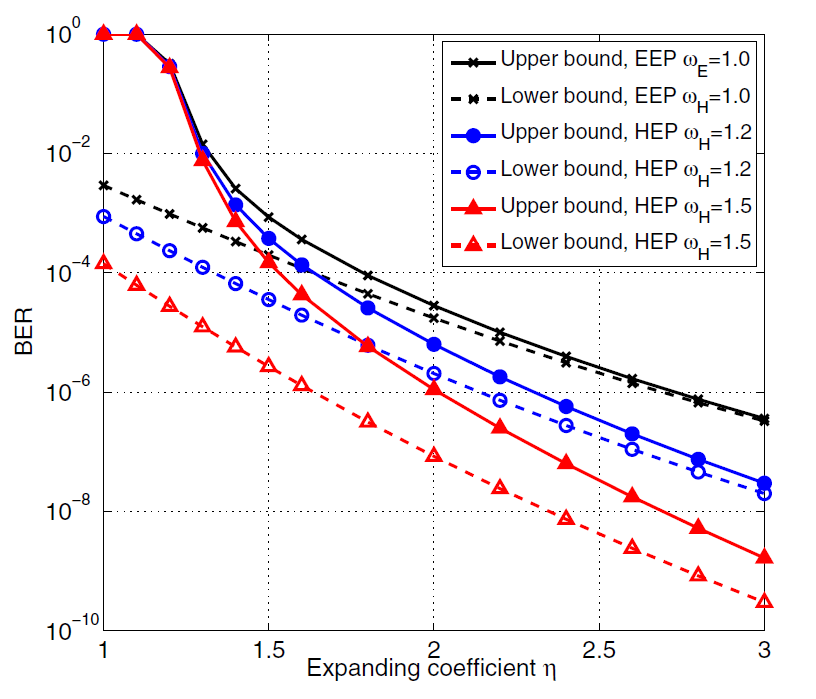
\includegraphics[width = 0.85\textwidth]{img/bounds_14a}
\end{minipage}
\begin{minipage}[c]{0.47\textwidth}
  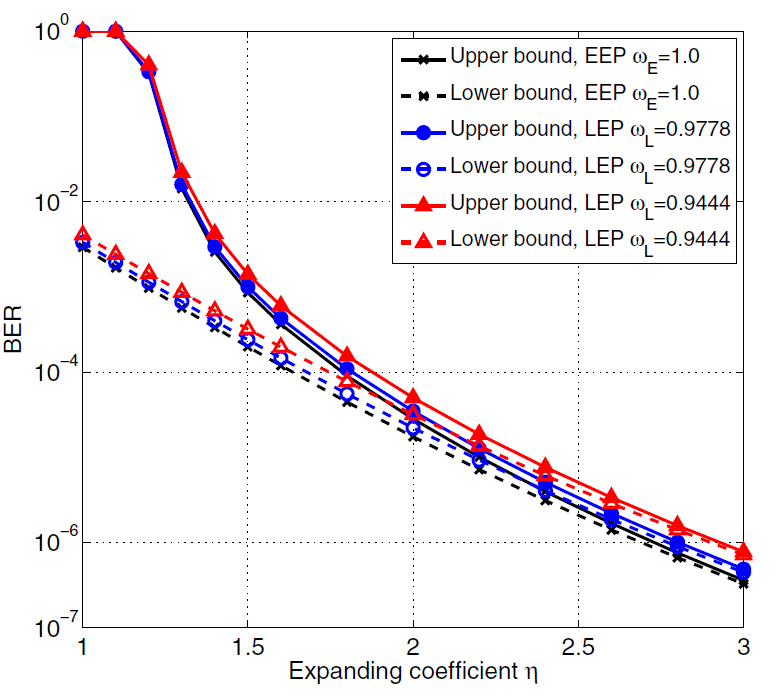
\includegraphics[width = 0.8\textwidth]{img/bounds_14b}
\end{minipage}
\caption{\footnotesize{BER performance bounds comparison of the \gls{uep} \gls{dnc} scheme based on fountain codes with \gls{ml} decoding over Rayleigh fading channels with $T=2$ and $K=100$. The left figure is for \gls{hep} group ($\alpha_H = 0.1$), the right one is for \gls{lep} group ($\alpha_L = 0.9$) Source \cite{Yue2014}}}
\label{fig:berLT}
\end{figure}
